\chapter{Main Modules}
\label{chTutorial}

The BATS agent architecture consists of several parts and layers. This
tutorial guides you through using these parts step by step. All lower
layers are independent of the higher layers, so if you do not need all
layers, you can skip the later sections. For instance, if you are only
interested in an easy interface with the simulation server, reading
section \ref{secSocketComm} will suffice. If you want to start quickly
with a working agent, you can skip until section
\ref{secHumanoidAgent} for now. However, the agent template described
there is based on the elements described in the sections before that,
so be sure to read those too at some time, to fully understand how
your agent works.

\begin{figure}
	\centering
	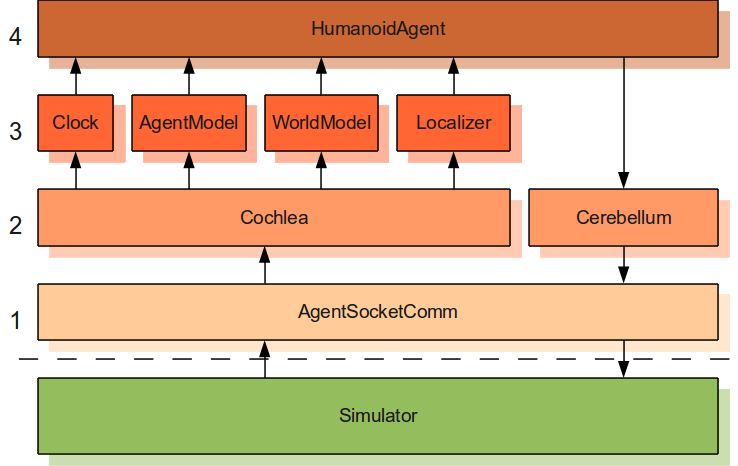
\includegraphics[width=0.7\textwidth]{libbats.png}
	\caption{{\tt libbats} modules}
	\label{fig:libbats}
\end{figure}

The main {\tt libbats} modules and their relations are shown in
Fig.~\ref{fig:libbats}. As you can see, they can be divided into
several layers:
\begin{description}
\item[1: Low level communication] As discussed in chapter
  \ref{chSimspark}, communication between the simulator and an agent
  is done using an ASCII, S-expression based protocol through a TCP/IP
  connection. The {\tt AgentSocketComm} module handles setting up this
  connection, reading and writing messages, and parsing these messages
  into and from more managable data structures.
\item[2: Input and output integration] In the second layer, input and
  output is handled at a slightly higher level. On the input side, the
  {\tt Cochlea} extracts all data from the still text-based messages
  supplied by the {\tt AgentSocketComm} and turns that data into
  readily usable binary values. The {\tt Cerebellum} is used to gather
  control commands, work out contradictions if necesary and turn them
  into the text based structures that the {\tt AgentSocketComm}
  understands.
\item[3: Models] The 4 modules in the third layer use the data from
  the {\tt Cochlea} to update models of the current state of the
  world, i.e. the current time, the state of the agent's body, the
  state of the world and the game, and the location of all objects in
  the field.
\item[4: Intelligence] Finally, at the highest level, the actual
  intelligence of the agent is implemented. An instance of {\tt
    HumanoidAgent} has access to all information gathered in the
  different modules, decides upon actions based on this information,
  and submits these actions to the {\tt Cerebellum}.
\end{description}

In the following sections we will describe in more detail how each
module can be used. While doing so, we will encounter different helper
and utility classes. Please refer to later chapters for more details
on these. Also, again, for more information, make sure to read the
Doxygen documentation contained in the source.

\lstset{numbers=none}

\section{AgentSocketComm}
\label{secSocketComm}

\lstset{numbers=none}

As mentioned earlier, the lowest layer in the library manages the
communication with the simulation server. This communication is done
through TCP sockets and consists of S-expressions (predicates) that
the agent and server send back and forth. To make sure you don't have
to worry about what this stuff actually is and does, the library
offers you the {\tt AgentSocketComm}. This class handles the
connection to the server and sending, receiving and parsing of
messages. This section explains how to use this module. If you use the
{\tt HumanoidAgent} class, all this is done for you.

Before you can use {\tt AgentSocketComm}, you have to supply a host
name and a port number to connect to. When running the server on the
same computer as your agent, with default settings, these are
'localhost' and '3100'. After this is done, the first thing to do is
to open an actual connection by calling {\tt connect()}:
\begin{lstlisting}[frame=single]
AgentSocketComm& comm = SAgentSocketComm::getInstance();
comm.initSocket("localhost", 3100);
comm.connect();
\end{lstlisting}

Note that the {\tt AgentSocketComm} is a singleton, refer to later
chapters for information on what this is. The {\tt AgentSocketComm}
keeps two internal message queues, one for input and one for
output. These queues are filled and emptied, respectively, when
calling {\tt AgentSocketComm}'s {\tt update()} method. This call
blocks until new data is received from the server:
\begin{lstlisting}[frame=single]
comm.update();
\end{lstlisting}

SocketComm supplies several methods to place messages that should be
sent to the server into the output queue. First of all, you can build
your own predicate using the {\tt Predicate} and/or {\tt Parser}
classes \footnote{This method is not described in this manual. Look at
  the documentation of the respective classes for more info} and put
it directly into the queue by calling the send method:
\begin{lstlisting}[frame=single]
rf<Predicate> myPredicate = makeMyPredicate();
comm.send(myPredicate);
\end{lstlisting}
However, you can also leave the trouble of building the predicates to
{\tt AgentSocketComm} by using its {\tt make*Message()} methods. And
if you want it totally easy, use the {\tt init()}, {\tt beam()} and
{\tt move*()} methods, which not only build the predicates, but also
place the messages directly into the queue for you.

The input queue holds the messages received from the server. To check
whether there is a new message, you can call {\tt hasNextMessage}. To
extract the next message, you can use {\tt nextMessage()}:
\begin{lstlisting}[frame=single]
while (comm.hasNextMessage())
  rf<Predicate> message = comm.nextMessage();
\end{lstlisting}

To conclude and summarize this section, a typical way to have
successful communication with the server is presented here:
\begin{lstlisting}[frame=single]
// Get the AgentSocketComm, initialize and connect
AgentSocketComm& comm = SAgentSocketComm::getInstance();
comm.initSocket("localhost", 3100);
comm.connect();

// Create robot model
rf<Predicate> scene = new Predicate("scene");
scene->pushLeaf("rsg/agent/" + am.getRSG());
comm.send(scene);

// Wait for the first message from the server
comm.update();

// Identify yourself to the server
comm.init(0, "MyTeam");

// Main loop
while (true)
{
  comm.update();
  while (comm.hasNextMessage())
    handleMessage(comm.nextMessage());
}
\end{lstlisting}

\section{Cochlea}
\label{secCochlea}

\lstset{numbers=none}

The {\tt AgentSocketComm} parses the S-expressions that the agent
receives from the server into a {\tt Predicate} structure. However, to
extract useful data you still have to dig through these
structures. The {\tt Cochlea} offers a layer over the {\tt
  AgentSocketComm} to extract information from the predicates received
from the server and present it in an easily accessible way.

Before using the Cochlea you have to initialize some parameters. You
have to let it know what the name of your team is, so it can tell team
mates and opponents apart:
\begin{lstlisting}[frame=single]
Cochlea& cochlea = SCochlea::getInstance();
cochlea.setTeamName("MyTeam");
\end{lstlisting}

Next you have to set up translations for joint-angle sensors. The {\tt
  Cochlea} uses internal names for these, that may not be the same as
the names used in the messages sent by the server. These internal
names are "head1", "head2", "larm1" to "larm4" for the left arm,
"rarm1" to "rarm4" for the right and "lleg1" to "lleg6" and "rleg1" to
"rleg6" for the legs. The Nao robot used by the server for instance
uses names of the form "laj1" and "rlj3", so these have to be
translated:
\begin{lstlisting}[frame=single]
cochlea.setTranslation("laj1", "larm1");
cochlea.setTranslation("rlj3", "rleg3");
\end{lstlisting}
This way the Cochlea can handle different robot models. If you use the
{\tt AgentModel} module, this is done for you.

Now you can start using the {\tt Cochlea} by calling {\tt update()}
every time a new message is received by the {\tt
  AgentSocketComm}. This will integrate the information of the
message, after which you can request data with the {\tt getInfo()}
method, or one of the methods for more complex data:
\begin{lstlisting}[frame=single]
comm.update();
cochlea.update();
// Get the polar coordinates of the ball
Vector3D polarBallPos = cochlea.getInfo(
                          Cochlea::iVisionBall);
\end{lstlisting}

\section{Clock}
\label{secClock}

The {\tt Clock} is pretty straightforward: it tells the current time:
\begin{lstlisting}[frame=single]
double t = SClock::getInstance().getTime()
\end{lstlisting}

\section{AgentModel}
\label{secAgentModel}

The {\tt AgentModel} keeps a model of the agent's own state. It
keeps track of joint angles and data of other sensors, as well as some
higher level data, like the position of the Center Of Mass (COM). The
{\tt AgentModel} also needs some initialization before it can be
used. You have to tell it the uniform number of the agent, after which
you should call the {\tt initBody()} method:
\begin{lstlisting}[frame=single]
AgentModel& am = SAgentModel::getInstance();
am.setUnum(unum);
am.initBody();
\end{lstlisting}

This loads an XML configuration file that contains the names, sizes
and weights of the agent's body parts and joints. It also uses this
data to set up the translations for the {\tt Cochlea} for you, so you
don't have to do this by hand. If default settings are used, the
default configuration file {\tt conf.xml} is loaded, which is
installed with the library and which imports the {\tt nao\_mdl.xml}
file for each agent to get the description of the Nao robot model. For
more information on loading XML configuration files and the robot
model descriptions, see the documentation of the {\tt Conf} class.

After initialization, the {\tt AgentModel} is also ready to be updated
and used:
\begin{lstlisting}[frame=single]
comm.update();
cochlea.update();
am.update();

Vector3D com = am.getCOM();
\end{lstlisting}

\section{WorldModel}
\label{secWorldModel}

The raw data offered by the {\tt Cochlea} may not be directly usable
and perhaps you want to have some information that is deduced from
these facts. This is exactly what the {\tt WorldModel} is for. It for
instance gives the current game state and field size, but also higher
level information like which team should take the kick-off, or if
there is another player closer to the ball.

To start, the {\tt WorldModel} also needs to know the name of your
team for some of its capabilities:
\begin{lstlisting}[frame=single]
WorldModel& wm = WorldModel::getInstance();
wm.setTeamName("MyTeam");
\end{lstlisting}

Next, the model has to be updated at every cycle. The {\tt WorldModel}
extracts data from the {\tt Cochlea}, so make sure it is updated
before updating the {\tt WorldModel}:
\begin{lstlisting}[frame=single]
comm.update();
cochlea.update();
wm.update();

bool shouldWeKickOff = wm.weGetKickOff();
\end{lstlisting}

\section{Localizer}
\label{secLocalizer}

\begin{figure}
\centering
\subfigure[Agent]{
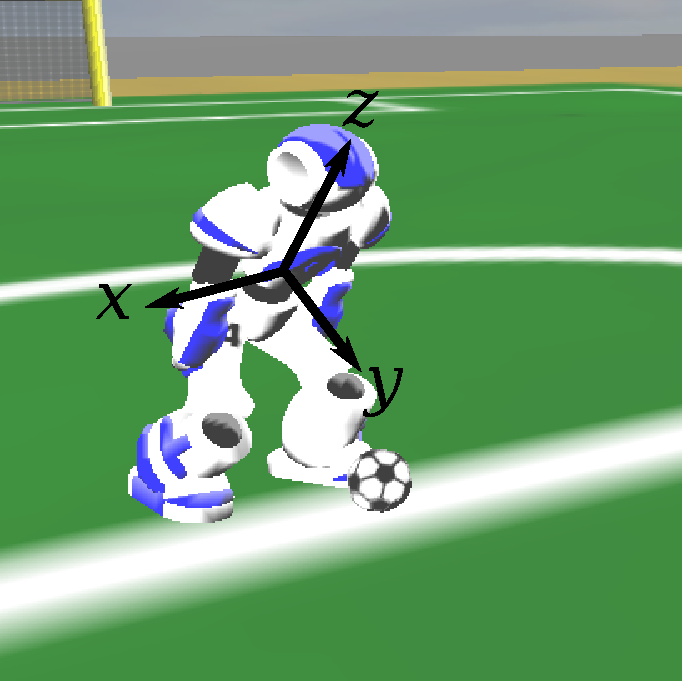
\includegraphics[width=.3\textwidth]{raw.pdf} \label{coordinatesraw}
}
\subfigure[Local]{
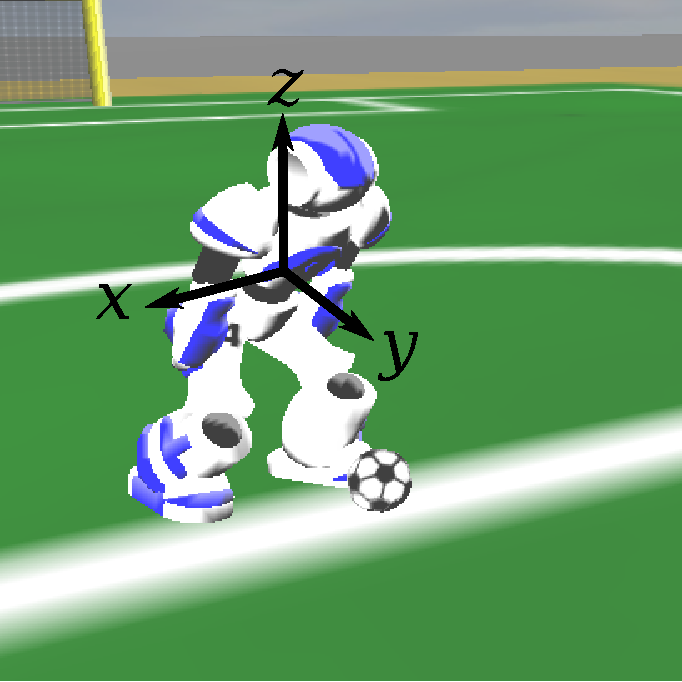
\includegraphics[width=.3\textwidth]{local.pdf} \label{coordinateslocal}
}
\subfigure[World]{
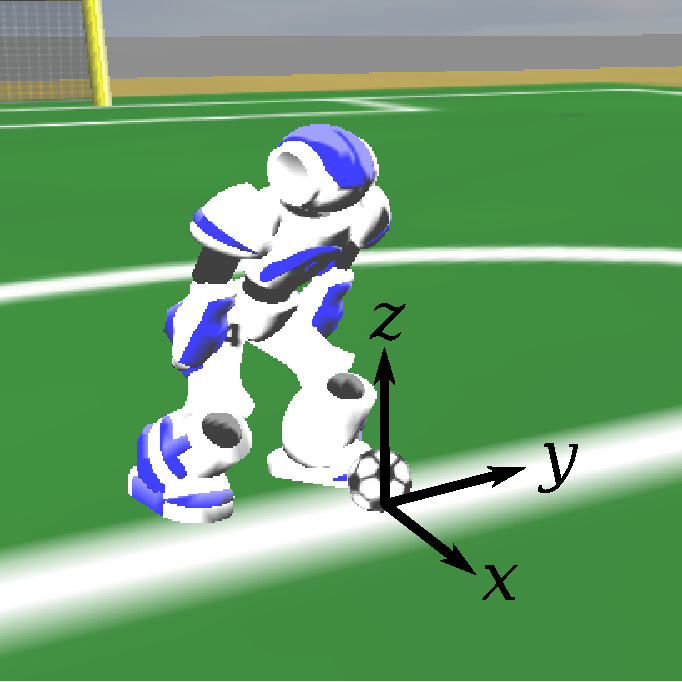
\includegraphics[width=.3\textwidth]{world.pdf}\label{coordinatesworld}
}
\caption{The coordinate systems used in {\tt libbats}: (a) Agent
  ('raw') coordinates, (b) local coordinates, and (c) global
  coordinates.}
\label{coordinates}
\end{figure}

The WorldModel provides the state of the game, such as the game time,
the gamestate, and the team name. However, often the agents will want
to know where they are, where the ball is, or where their opponents
are. This can be obtained through the {\tt Localizer}. To be able to
implement different localization methods, the {\tt Localizer} is an
abstract class from which all implementations are derived. One
realization of this class is provided in {\tt libbats}, called the
{\tt KalmanLocalizer}. As you might have guessed, this {\tt Localizer}
uses a Kalman filter to keep track of the locations of the player
itself and of other objects. At the start of the program, we have to
initialize the Localizer and tell it which implementation to use:
\begin{lstlisting}[frame=single]
SLocalizer::initialize<KalmanLocalizer>();
\end{lstlisting}

Like the other models, the update() member function of the {\tt
  Localizer} should be called each timestep to update the current
location estimates with new data from the {\tt Cochlea}. The other
member functions of the Localizer can be used to obtain the current
position of the agent itself, the ball, the other players, or objects
such as the goal posts and corner flags.

Within {\tt libbats}, several different coordinate systems are used
(see Fig.~\ref{coordinates}:
\begin{description}
\item[Agent/raw coordinates] The origin of this system is the center
  of the agent's torso. The positive x axis extends to the right,
  parallel to the line through the shoulders, the positive y axis
  forward out of the torso, and the positive z-axis upwards, through
  the center of the head. This system is used by the {\tt AgentModel}
  for the coordinates of body parts. Shown in
  Fig.\ref{coordinatesraw}.
\item[Local coordinates] The origin of the local coordinate system is
  also the center of the agent's torso, but the positive z axis of
  this system always points upwards, perpendicular to the field. So,
  the x and y axes always lie parallel to the field, pointing right
  and forward respectively. This is one of the systems used by the
  {\tt Localizer} and is the most intuitive to use to determine 'in
  front of me/to the side of me/above of me' relations. Shown in
  Fig.\ref{coordinateslocal}.
\item[World coordinates] The world coordinate system is fully
  independent of the agent's location and orientation. Its origin is
  the center of the field, the positive x axis points to the center of
  the opponent's goal, the positive y-axis to the left when looking
  along the x axis, and the positive z axis points up, perpendicular
  to the field. This is the second system that is used by the {\tt
    Localizer} and is the best one to use to determine global
  relations. Shown in Fig.\ref{coordinatesworld}.
\end{description}

\section{Cerebellum}
\label{secCerebellum}

The {\tt Cochlea} takes the trouble of having to deal with raw
predicates on the input side. On the output side the {\tt Cerebellum}
is there for you. It supplies more useful structures to define actions
and the possibility to integrate actions from different sources in
your agent. The {\tt Cerebellum} defines the {\tt Action} substructure
and a few of its derivatives with which you can make new actions. At
the moment there are 5 different action types available:
\begin{description}
\item[{\tt MoveJointAction}] Move a hinge joint or one axis of a universal joint.
\item[{\tt MoveHingeJointAction}] Move a hinge joint.
\item[{\tt MoveUniversalJointAction}] Move both axes of a universal joint.
\item[{\tt BeamAction}] Beam to a certain position.
\item[{\tt SayAction}] Shout something.
\end{description}
If you don't understand the difference between hinge and universal
joints, don't worry. Just use {\tt MoveJointAction}s and let the {\tt
  Cerebellum} handle the rest.

The {\tt Cerebellum} again is a singleton that can be retrieved by
calling \\ {\tt SCerebellum::getInstance()}, after which you can add
actions to it. After all the sub parts have added their actions, you
can call {\tt outputCommands()} to send them through an {\tt
  AgentSocketComm}:
\begin{lstlisting}[frame=single]
Cerebellum& cer = SCerebellum::getInstance();

rf<MoveJointAction> action =
  new MoveJointAction(Types::LLEG1, 0.1);
cer.addAction(action);

cer.outputCommands(comm);
\end{lstlisting}
When more than one action is supplied for a joint, the angular
velocities will be added together before sending the actions to the
server.

\section{HumanoidAgent}
\label{secHumanoidAgent}

Now you have learned about how to initialize, update and maintain the
several models of the library, you will learn how to forget all
that. The {\tt HumanoidAgent} class does this all for you. It connects
the {\tt AgentSocketComm}, initializes the {\tt Clock}, {\tt
  AgentModel}, {\tt WorldModel} and {\tt Localizer} and updates all
modules in the correct order at every cycle. See chapter
\ref{chQuickstart} to learn how to use this class to set up your own
agent.


\section{XML Configuration}
\label{sec:xml-configuration}

The \libbats library comes with an XML based configuration framework,
to make it easier to set parameters at runtime without having to
recompile, either globally, for a specific module, or for specific
agents. The library comes with a minimal configuration file, at `{\tt
  xml/conf.xml}' that is loaded by default, unless you pass a
different file path to the {\tt HumanoidAgent} constructor. You should
base your own configuration file on this one, as it contains the minimally necessary items:
\begin{itemize}
\item A correct XML header, and a root `conf' element that includes
  that XInclude namespace.
\item The inclusion of the XML file describing the robot model.
\item A `player-class' element for each possible player class, where
  by default each class index corresponds to a uniform number.
\end{itemize}
This is sufficient configuration for \libbats internally. The
following sections describe which classes to use and how to format
your XML file to use the configuration framework in your own code.

\subsection{{\tt Conf}}
\label{sec:tt-conf}

The direct interface to the configuration file is provided by the {\tt
  Conf} class. It is again a singleton, to get a reference to it use:
\begin{lstlisting}[frame=single]
Conf& conf = Conf::getInstance();
\end{lstlisting}
It is used to parse the XML file (which is done for you
if you use the {\tt HumanoidAgent} class), and gives direct access to
it through XPath expressions. However, usually you want to use the
higher level {\tt getParam} methods on it to get configuration
parameters. There are two variants, both templated:
\begin{description}
\item[\tt T getParam(string name, T def)] Use this to get global parameter
  values, that are defined in a `parameters' element directly under
  the `conf' root element. The first argument gives the name of the
  parameter to look for, the second gives a default value to return if
  the parameter is not found in the configuration file. Note that the
  type of this second argument also determines the type of the return
  value. Consider the following statements, given the the example
  configuration file in listing \ref{confxml}:
\begin{lstlisting}[frame=single]
double foo = conf.getParam("foo", 2.0);
string bar = conf.getParam("bar", string("unknown"));
\end{lstlisting}
  After this, {\tt foo == 1.0}, as defined in the XML file, and {\tt
    bar == "unknown"}, because there is no global parameter `bar' set
  in configuration. Note that to read a string parameter you have to
  explicitly pass a {\tt std::string} value as second argument.

  Within the library a few parameters are read with this
  method. Currently these only consist of field dimensions, and
  whether the server is restarted for half time or not. To override
  the default values for these, use the following format:
\begin{lstlisting}[frame=single,language=xml]
<conf xmlns:xi="http://www.w3.org/2003/XInclude">
  <parameters>
    <fieldlength>30</fieldlength>
    <fieldwidth>20</fieldwidth>
    <goalwidth>2.1</goalwidth>
    <goalheight>0.8</goalheight>
    <penaltyxlength>1.8</penaltyxlength>
    <penaltyylength>3.9</penaltyylength>
    <numberofplayers>11</numberofplayers>
    <halftimerestart>1</halftimerestart> <!-- 1 = true, 0 = false -->
  </parameters>
  
  ...
\end{lstlisting}
  If these parameters are missing, default values will be loaded
  (which are the values shown above).

\item[\tt T getParam(unsigned playerClassIdx, string name, T def)] The
  second variant takes a player class index as an additional
  parameter, to fetch parameters specific to a certain player. Again
  given listing \ref{confxml}, consider the following statements:
\begin{lstlisting}[frame=single]
string bar1 = conf.getParam(1, "bar", string("unknown"));
string bar2 = conf.getParam(2, "bar", string("unknown"));
string bar3 = conf.getParam(3, "bar", string("unknown"));
\end{lstlisting}
  The values of {\tt bar1}, {\tt bar2}, and {\tt bar3} will be
  ``attacker'', ``defender'', and ``unknown'', respectively.

  What you use as an index is completely up to you, but a sensible
  choice is the uniform number, which you can get from the {\tt
    AgentModel}. The library also provides a simple framework to start
  you off with more dynamic player class selection, through the
  interface supplied by the {\tt PCSelector} class. You can inherit
  from this class to create your own method of selecting the role of a
  player, then choose it when initializing the {\tt PCSelector}
  singleton. Currently only one implementation is included in
  \libbats, the {\tt UnumPCSelector}, which simply returns the uniform
  number. It can be initialized and used as follows:
\begin{lstlisting}[frame=single]
SPCSelector::initialize<UnumPCSelector>();
...
conf.getParam(SPCSelector::getInstance().getPlayerClass(), "foo", 2.0);
\end{lstlisting}

\end{description}

\begin{lstlisting}[float,caption={\tt conf.xml},label=confxml,frame=single]
<?xml version="1.0" encoding="ISO-8859-1"?>
<conf xmlns:xi="http://www.w3.org/2003/XInclude">  
  <xi:include href="nao_mdl.xml"/>

  <parameters>
    <foo>1</foo>
  </parameters>

  <myclass id="inst1">
    <foo>10</foo>
  </myclass>

  <player-class index="0"/>

  <player-class index="1">
    <parameters>
      <bar>attacker</bar>
    </parameters>
  </player-class>

  <player-class index="2">
    <parameters>
      <bar>defender</bar>
    </parameters>
  </player-class>

  <player-class index="3"/>

  <player-class index="4"/>

  <player-class index="5"/>

  <player-class index="6"/>

  <player-class index="7"/>

  <player-class index="8"/>

  <player-class index="9"/>

  <player-class index="10"/>

  <player-class index="11"/>
</conf>  
\end{lstlisting}

\subsection{{\tt Configurable}}
\label{sec:tt-configurable}

Beyond direct access through the {\tt Conf} class, you can make your
own classes configurable by having them extend the.. {\tt
  Configurable} class. When doing so, your class' constructor must
pass two things to the constructor of {\tt Configurable}: a tag name
and an ID string. These are then used to find the value of parameters
when calling the {\tt getConfParam} method. 

\begin{lstlisting}[float,caption={\tt Configurable} example,label=configurableexample,frame=single]
#include <libbats/Configurable/configurable.hh>

class MyClass : public bats::Configurable
{
public:
  MyClass(std::string const& id) : bats::Configurable("myclass", id)
  {
    d_foo = getConfParam("foo", 1.0);
  }

  double getFoo() const { return d_foo; }
private:
  double d_foo;
};
...
MyClass inst1("inst1");
MyClass inst2("inst2");

cout << inst1.getFoo() << endl; // Output: 10
cout << inst2.getFoo() << endl; // Output: 1
\end{lstlisting}

Listing \ref{configurableexample} gives a usage example, where the
parameter for the first instance is fetched from the configuration
file, whereas the second resorts to the default value.

%%% Local Variables: 
%%% TeX-master: "libbatsmanual"
%%% End: 
